\section{Background}
\label{sec:background}

Our work lies at the confluence of three distinct areas of networking and distributed systems: Zero-Configuration Networks (Zeroconf), in-browser Web servers, and fault tolerance.

\begin{figure}[h]
      \centering
      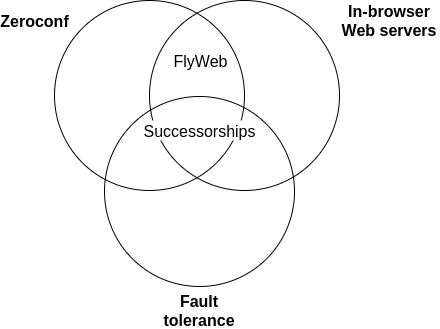
\includegraphics[keepaspectratio,width=6cm]{shippy-intersections}
      \label{fig:stack}
\end{figure}

\subsection{Zeroconf}
\label{sub:background_zeroconf}

Hosts connected to a network rely on maintaining a common consensus on such basic matters as addressing and name resolution, if they are to have any hope of communicating over that network.
This need is often fulfilled by specially-designated configuration servers, such as DHCP or DNS servers.
However, such servers can be absent in common networking situations, such as \textit{ad hoc} networks.
In such cases, it remains desirable for hosts to handle these matters in a seamless and cross-platform fashion, without the need for manual configuration.
This is the problem addressed by the group of protocols referred to as Zeroconf, short for ``Zero Configuration Networking''.
Although the term is sometimes used more broadly to designate any suite of technologies that seeks to address this problem, we observe the more specific meaning established by the former IETF Working Group by the same name\footnote{http://www.zeroconf.org/}.
Zeroconf protocols solve the problems of address allocation (IPv4LL), address queries (mDNS), and network service discovery (DNS-SD), specifically when hosts share a direct link (be it logical or physical).
 
\textbf{Address allocation.}
When a client running DHCP connects to a network managed by a DHCP server, the server assigns to the client an available IP address in the local network.
A Zeroconf protocol called IPv4LL (short for IPv4 Link Local) is intended for use in the absence of such a server.
IPv4LL specifies how a connecting client may check directly the availability of an IPv4 address before claiming it on that local network, and specifies how to resolve conflicts between two or more hosts having claimed the same address~\cite{rfc3927}.
IPV4LL has been integrated into consumer operating systems and printers since the early 2000s.

\textbf{Address queries.}
A name server can be used on a local network to maintain a mapping of logical names to IP addresses.
In the absence of such a server, a Zeroconf protocol called mDNS (short for ``multicast DNS'') can be used to formulate address queries on the local network.
As per its name, mDNS broadcasts these queries onto the local network rather than directing them to a single server; it also includes a mechanism to resolve naming conflicts~\cite{rfc6762}.
mDNS aims to handle any type of record lookup that could be handled by a DNS server, not just name-to-address lookups.
mDNS has grown steadily in popularity amongst networked devices; implementations of mDNS include Apple Bonjour, Spotify Connect, Philips Hue, Google Chromecast, and Avahi (an open-source implementation for Linux).

\textbf{Service discovery.}
Once connected to a network, a host may wish to learn about the services offered by the other devices connected to the network, such as printing or media streaming.
In a centrally-administered network, this may be accomplished by a directory server, such as a DNS server.
However, when such a server is lacking, the Zeroconf protocol called DNS-SD (``DNS service discovery'') leverages the ability to make distributed DNS queries provided by mDNS, to register, enumerate, and resolve local network services~\cite{rfc6763}.


%\subsection{Zeroconf Networking}
\label{sub:background_zeroconf_networking}

Zero-configuration networking (``zeroconf'') is a combination of protocols that aim to automatically discover computers or peripherals in a network without any central servers or human administration. 
Zeroconf networks have two major components that provide {\it (i)} automatic assignment of IP addresses and host naming (mDNS), and {\it (ii)} service discovery (DNS-SD).

When a device enters the local network, it assigns an IP/name pair to itself and  multicasts this pair to the local network, resolving any name conflicts that may occur in the process. 
IP assignment considers the link-local domain address, drawing addresses from the IPv4 169.254/16 prefix; once an IP address is selected, a host name with the suffix ``.local'' is mapped to that IP~\cite{rfc6762}. 
As devices are mapped to IPs/host names, their available services are discovered using a combination of DNS PTR, SRV, and TXT records~\cite{rfc6763}; their services can then be requested by other devices.

The design focus of zeroconf networking protocols is smooth assignment of names and discovery of services without the configuration tasks normally present in network infrastructure.
Our aim is to build upon the appealing features of zeroconf networks by making them fault tolerant.
This property is desirable in any scenario where network services need to remain stable even when the server node disconnects.
In the zeroconf setting, we anticipate that the hassle-free set-up will be complemented naturally by a system that enables a service to be provided in uninterrupted fashion, even when the server node disconnects.


%\subsection{Zeroconf Examples}
\label{sub:background_zeroconf_examples}

The concept of creating local ad-hoc networks with very little configuration has been under development for several years.

Published in 2008, Universal Plug and Play (UPnP) is one of the more widely-deployed examples of a zero-configuration networking technology in use today. 
It consists of a set of networking protocols developed to facilitate interaction with services offered by any networked device on a local network.
Since it leverages common protocols (HTTP/XML/SOAP on UDP/IP) and is agnostic to the link medium, it is truly cross-platform, extending not only to phones and laptops but also to printers, WiFi routers, and audio-visual equipment, to name a few examples.
Many consumer devices currently come with UPnP capability built in.
However, UPnP has been criticized for being insecure (by default, it assumes that all devices on the local network can be trusted, and so does not provide any means for authentication) and unscalable (due to use of multicast for service discovery).

More recently in 2017, as part of its \textit{Nearby} project, \textit{Google} released its \textit{Connections} API, which enables Android devices in close proximity to one another to communicate in a peer-to-peer fashion.\footnote{https://developers.google.com/nearby/connections/overview}
This is done over a seamless mix of Bluetooth, BLE, and WiFi hotspots.
Unfortunately, Google has only made this API available on the Android platform; we seek a solution that is truly cross-platform.


\subsection{In-Browser Web Servers}
\label{sub:background_in_browser_web_servers}

More recently, a number of technologies have emerged to enable Web servers to be deployed entirely from within Web browsers.
Such technologies have the appeal that they simplify the process of serving Web content, thus potentially expanding the breadth of users capable of doing so.
For example, Opera Unite\footnote{http://help.opera.com/Windows/12.10/en/unite.html}, Web Server Chrome\footnote{https://github.com/kzahel/web-server-chrome}, PeerServer\footnote{http://www.peer-server.com/}, and FlyWeb\footnote{http://flyweb.github.io/} all enable browser applications to publish fully functioning Web servers.

HTTP servers running on hosts that usually access the Web as clients face a few challenges not normally encountered by those running on dedicated server machines.
For example, they must be properly configured to circumvent firewalls, and they must ensure that other clients have a way of finding out their IP address.
Most in-browser web server frameworks address these issues, albeit in a variety of different ways; we discuss how the FlyWeb project achieves this below, and refer the reader to Section \ref{sec:related_work} for details on other approaches.

\textbf{FlyWeb.}
The FlyWeb project, developed by the Mozilla Firefox community, addresses the problem of advertising and discovering in-browser Web services in the particular environment of local networks, by leveraging Zeroconf service advertisement and discovery.
To this end, FlyWeb provides two key pieces of functionality: 
\textit{(i)} an implementation of mDNS, allowing those services to advertise their name and address to peers on the local network, and 
\textit{(ii)} a FlyWeb service discovery menu, which uses a built-in implementation of DNS-SD to enumerate locally-discovered services.
The goal is for devices on a local network to be able to stream applications and content to one another using widely available Web technology.\footnote{https://hacks.mozilla.org/2016/09/flyweb-pure-web-cross-device-interaction/}
FlyWeb was released in mid-2016, but is no longer actively maintained as of August 2017.

A different challenge facing in-browser Web servers is that their availability is limited by the host machine's uptime.
Dedicated server machines are usually non-mobile and optimized for availability; however, the class of devices that can run a Web browser is much wider, including mobile devices, hence posing a challenge to service availability.
To the best of our knowledge, at the time of writing, none of the currently-existing technologies address the issue of recovering from disruptions of server availability for in-browser Web services.



%\subsection{FlyWeb}
\label{sub:background_flyweb}

The \textit{FlyWeb} project\footnote{http://flyweb.github.io/}, developed by the Mozilla Firefox community, aims to bring the convenience of Zeroconf functionality to the versatility and ubiquity of Web applications.
FlyWeb enables scripts in the browser to start local Web servers, and to have those servers be locally discoverable and addressable by providing a built-in implementation of mDNS and DNS-SD.
It also provides a browser extension to discover and easily connect to local FlyWeb services.
The goal is for devices on a local network to be able to stream applications and content to one another using widely available Web technology.\footnote{https://hacks.mozilla.org/2016/09/flyweb-pure-web-cross-device-interaction/}
FlyWeb was released in mid-2016, but is no longer actively maintained as of August 2017.


\subsection{Replication}
\label{sub:background_replication}

Fault tolerance and reliability in distributed systems with client-server architecture are generally achieved by data replication: information is shared on redundant server replicas such that any replica can become the new master if the current master fails. While improving system artifacts like fault-tolerance, reliability and availability, replication can come at the cost of performance: depending on the required operations in the system for replication, system performance can suffer significant bottlenecks. Different models of replication have been proposed to trade consistency for performance, resulting in different levels of consistency as a design choice for the target system. Traditionally, two strategies of replication are distinguished: \textit{active replication} and \textit{passive replication}. A third type of replication, \textit{lazy replication}, was later introduced and is gaining more attention recently. The following paragraphs describe these three types of replication.

\textbf{Active replication.} The first strategy (also called \textit{primary-backup} or \textit{master-slave}), requests to the master replica are processed to all other replicas. Given the same initial state and request sequence, all replicas will produce the same response sequence and reach the same final state. Active replication has become most prominent with the introduction of the State Machine Replication model which was introduced in the 1980s \cite{Lamport:1984} and later refined in \cite{Schneider:1990}. It is based on the concept of distributed consensus with the goal of reliably reaching a stable state of the system in the presence of failures. While providing small recovery delay after failures due to an imposed total order of state updates, computation performance can suffer tremendous bottlenecks since updates must be sequentially propagated through all replicas.

\textbf{Passive replication.} The second strategy (also called \textit{multi-primary} or \textit{multi-master} scheme) relaxes sequential ordering: clients communicate with a master replica and updates are forwarded to backup replicas. Computation performance is improved with this pattern since all computation takes place on the master replica and only the results are propagated. The downside of the approach is that more network bandwidth is required if updates are large. Since the primary replica represents a single point of entry to clients with this approach, there must be some kind of distributed concurrency control in order to reliably restore state when the primary fails. This makes the implementation of this approach more complex and recovery potentially slower. One promising approach of passive replication is Chain Replication \cite{VanRenesse:2004}. Whereas traditional topologies resemble stars with the master replica at the center, this approach forms a chain of replicas with the primary being the tail of the chain. This model aims at providing high availability without sacrificing strong consistency. The main advantage is that reads can address one end of the chain and writes the other. While recovery of failing tail or head servers is simple, recovery of failing middle-servers is complex.

\textbf{Lazy replication.} A third strategy of replication was proposed in 1990: \textit{lazy replication} \cite{Ladin:1990,Ladin:1992} (also called \textit{optimistic replication}) aims at providing highest possible performance and availability by sacrificing consistency significantly. With this approach, replicas periodically exchange information, tolerating out-of-sync periods but guarantee to catch up eventually. While the traditional approaches guarantee from the beginning that all replicas have the exact same state at any point in time, lazy replication allows states to diverge on replicas, but guarantees that the states converge when the system quiesces for some time period. In contrast to the strong consistency models used in the traditional approaches, lazy replication is based on eventual consistency which has gained more attention recently, in particular in online editing platforms, NoSQL cloud databases and big data \footnote{http://www.oracle.com/technetwork/consistency-explained-1659908.pdf, accessed 2017-10-08}. Eventual consistency is the weakest consistency model, providing no guarantee for safety as long as replicas have not converged. Rather, it "push[es] the boundaries of highly available systems" \cite{Bailis:2013}. The introduction of \textit{conflict-free replicated data types} \cite{Shapiro:2011} aimed at a stronger model of eventual consistency: any two replicas that receive the same updates, no matter the order, will be in the same state. CFDTs are categorized in operation-based (only update operation is propagated) and state-based (full state is propagated). A number of CFDTs have been suggested, among them are sets, maps and graphs. It is important to mention that all eventual consistency models impact the application designer since she has to determine what level consistency is sufficient for the specific application.


% TODO (PTC): The broader term for what we want to implement is "failover", except in a distributed setting. Look into existing literature on this term.
